\section{图的连通度}
\subsection{割边、割点和块}

\subsubsection{割边及其性质}

\begin{definition}
	设$e$是图$G$的一条边,若\colorbox{yellow}{$\omega(G-e)>\omega(G)$},则称$e$为$G$的\textcolor{red}{割边}
\end{definition}

\begin{theorem}
	边 $e$ 是图$G$的割边当且仅当 $e$ 不在$G$的任何圈中.
\end{theorem}

\begin{corollary}
	$e$为连通图$G$的一条边,如果$e$含于$G$的某圈中,则$G-e$连通.
\end{corollary}

\begin{example}
	\label{yyhng}
	求证: (1) 若$G$的每个顶点的度数均为偶数,则$G$
	没有割边; (2) 若$G$为$k$正则二部图$(k\geq 2)$,则$G$无割边.
\end{example}
\begin{proof}
(1) 若不然,设$e=uv$ 为$G$的割边. 则$G-e$的含有
顶点$u$(或$v$)的那个分支中点$u$(或$v$)的度数为奇,而其余点
的度数为偶数,与“度数为奇数的顶点的个数为偶数”相矛盾!

(2) 若不然,设$e=uv$ 为$G$的割边. 取$G-e$的其中一个分
支$G_1$, 显然,$G_1$中只有一个顶点的度数是$k-1$,其余点的度
数为$k$. 并且$G_1$仍然为偶图.

假若$G_1$的两个顶点子集包含的顶点数分别为$s$与$t$,并且$s$包含顶点度为$k-1$的点,那么有:
$ks - 1=|E(G_1)|=kt$. 但是因$k\geq 2$, 所以等式不能成立!
\end{proof}
\begin{note}
	{ 割点有两类,一类是自环,一类是破坏连通性的点}.
\end{note}


\subsubsection{割点及其性质}

\begin{definition}
在$G$中,如果$E(G)$可以划分为两个非空子集$E_1$
与$E_2$,使$G[E_1]$和$G[E_2]$以点$v$为公共顶点,称$v$为$G$的一个
\textcolor{red}{割点}.
\end{definition}
\begin{theorem}
$G$无环且非平凡,则$v$是$G$的割点,当且仅当
\[
\colorbox{yellow}{$\omega(G-e)>\omega(G)$}
\]
\end{theorem}

\begin{theorem}
$v$ 是树$T$的顶点,则$v$是割点,当且仅当$v$是树
的分支点.
\end{theorem}

\begin{theorem}
设$v$是无环连通图$G$的一个顶点,则$v$是$G$的割
点,当且仅当$V(G-v)$可以划分为两个非空子集$V_1$与$V_2$,使
得对任意$x \in V_1, y \in V_2$, 点$v$在每一条$(x,y)$路上。
\end{theorem}

\begin{example}
	求证:无环非平凡连通图至少有两个点不是割点.
\end{example}
\begin{proof}
	由于 $G$ 是无环非平凡连通图,所以存在非平凡生成树.非平凡生成树至少两片树叶,它
	们不能为生成树的割点.显然,它们也不能为 $G$ 的割点.
\end{proof}
\begin{note}
	非平凡树一定有割边,不一定有割点 $(K_2)$.
\end{note}
\begin{theorem}[割点与割边关系]
	\begin{enumerate}
		\item 没有割点 \( \nRightarrow \) 没有割边 \( \left(K_{2}\right) \).
		\item 有割边 \( \nRightarrow \) 有割点 (八字形的图).
	\item 阶数 \(n \geq 3 \) 的无环连通图, 有割边 \( \Rightarrow \) 有割点.
		\item 阶数 \( n\geq 3 \) 的无环连通图, 有割点 \( \nRightarrow  \) 有割边.
	\end{enumerate}
\end{theorem}




\subsubsection{块及其性质}
\begin{definition}
\colorbox{yellow}{没有\textcolor{red}{割点}的连通图称为是一个块图}
\end{definition}

\begin{theorem}
	若$|V(G)|\geq 3$,则$G$是块,当且仅当$G$无环且任意
	两顶点位于同一圈上.
\end{theorem}

\begin{theorem}
	点$v$是图$G$的割点当且仅当$v$至少属于$G$的两个不
	同的块.
\end{theorem}
\begin{note}
	\begin{enumerate}
		\item $(m=1)$块,要么是割边,要么是环;
		\item $(k = 1)$块要么是孤立点,要么是环;
		\item $(k\geq 2)$块无环;
		\item $(k\geq 3)$块无割边,无自环,有圈.
	\end{enumerate}
\end{note}



\noindent {\bfseries \textcolor{ecolor}{块割点树:}}

\begin{figure}[H]
	\small
	\centering 
	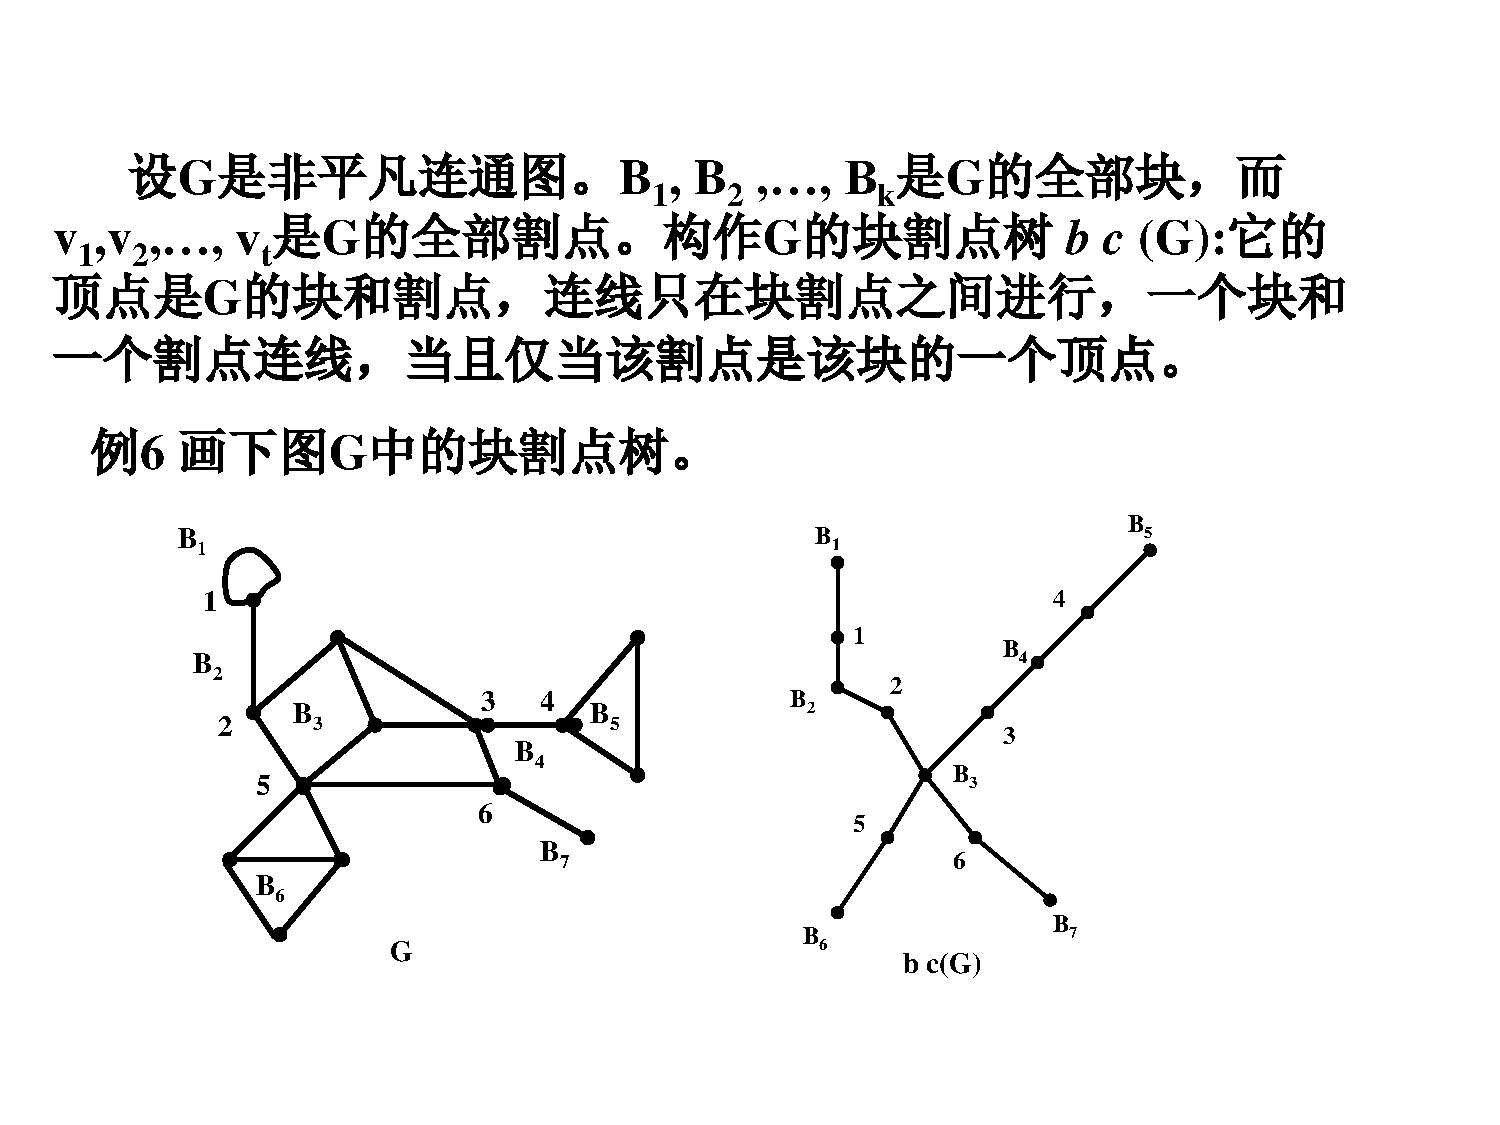
\includegraphics[scale=0.42]{image/CH3_kuai.pdf}  
	%\caption{信息包结构} 
	\label{figk1ik}  
\end{figure}

\subsection{连通度}
\begin{definition}
	\begin{enumerate}
		\item 给定\colorbox{yellow}{连通图}$G$,设\colorbox{yellow}{$V^{'}\subseteq V(G)$},若$G -V^{'}$ 不连通,称$V^{'}$为$G$的一个点割集,含有$k$个顶点的点割集
		称为\colorbox{yellow}{\textcolor{red}{$k$顶点割}}.$G$中点数最少的顶点割称为\colorbox{yellow}{\textcolor{red}{最小顶点割}}.
		\item 在$G$中,若\colorbox{yellow}{存在}顶点割,称$G$的最小顶点割的顶
		点数称为$G$的\colorbox{yellow}{\textcolor{red}{连通度}};否则称$n-1$为其点连通度.$G$的点连通度记为\colorbox{yellow}{$k(G)$}, 简记为$k$.若$G$不连通,\colorbox{yellow}{$k(G)=0$}.
		
		\item 给定\colorbox{yellow}{连通图}$G$,称使$G-E^{'}$不连通的$G$的边子集$E^{'}$为$G$的割边集,含有$k$条边的边割集称为\colorbox{yellow}{\textcolor{red}{$k$边割}}.$G$中边数最少的边割称为\colorbox{yellow}{\textcolor{red}{最小边割}}.
		\item 在$G$中,最小边割集所含边数称为$G$的\colorbox{yellow}{\textcolor{red}{边连通
		度}}.边连通度记为\colorbox{yellow}{$\lambda(G)$}.若$G$不连通或$G$是平凡图,则
		定义\colorbox{yellow}{$\lambda(G)=0$}.
		\item  若一个图的\colorbox{yellow}{\textcolor{red}{连通度}}至少为$k$,则称该图是\colorbox{yellow}{\textcolor{red}{$k$连通的}}(\textcolor{red}{$k(G)\geq k$});若一个图的\colorbox{yellow}{\textcolor{red}{边连通度}}至少为$k$,则称该图是\colorbox{yellow}{\textcolor{red}{$k$边连通的}}(\textcolor{red}{$\lambda(G)\geq k$}).
\end{enumerate}
\end{definition}

\begin{note}
		\begin{enumerate}
		\item $k$ 连通:要想破坏连通性,至少要删去 $k$ 个点.
		\item $K_2$ 连通、无割点,但连通度为 1($k$通度的图不一定存在$k$点割).
		\item $k$ 边连通:要想破坏连通性,至少要删去 $k$ 条边.
		\item \textcolor{red}{$k$ 连通一定是 $k$ 边连通的}.
		\item $k(K_n)=\lambda(K_n)=n-1$.
		\item $k(C_n)=2(n\geq 3); \lambda(C_n)=2(n\geq2)$. $C_n$为$n$圈.
	\end{enumerate}
\end{note}

\begin{theorem}[惠特尼1932]
	\label{huiteni}
	对任意图$G$,有:
	\[
	\colorbox{yellow}{$k(G)\leq \lambda(G) \leq \delta(G)$}
	\]
\end{theorem}


\begin{theorem}
	设$G$是$(n, m)$连通图,则:
	\[
	\colorbox{yellow}{$k(G)\leq \left[\dfrac{2m}{n}\right]$}
	\]
\end{theorem}
\begin{proof}
	由握手定理得$2m = \sum d(v) \geq n \delta \Rightarrow \delta \leq \frac{2m}{n}$
	
	由定理\ref{huiteni}得$k(G)\leq \delta$,考虑到$k(G)$是整数,所以
	\[
		k(G)\leq \left[\frac{2m}{n}\right]
	\]
\end{proof}


\begin{lemma}
	\textcolor{red}{设$G$是$n$阶简单图,若$\delta(G)\geq\left[\frac{n}{2}\right]$,则$G$连通}.
\end{lemma}
\begin{proof}
	若$G$不连通,则$G$至少有两个连通分支,于是,至
	少有一个分支$H$满足$|V(H)|\leq \left[\frac{n}{2}\right]$.因为$G$是简单图,从而
	\[
	\varDelta(H) \leq \left[\dfrac{n}{2}\right]-1  <\left[\dfrac{n}{2}\right]
	\]
	于是
	\[
	\delta(G) \leq \delta(H)\leq \varDelta(H) < \left[\frac{n}{2}\right]
	\]
这与已知矛盾,所以$G$必连通.
\end{proof}

\begin{theorem}
		设$G$是$n$阶简单图,对正整数$k< n$,若
	\[
	\delta(G)\geq \dfrac{n+k-2}{2}
	\]则$G$是$k$连通的.
\end{theorem}
\begin{theorem}
		\textcolor{red}{设$G$是$n$阶简单图,若$\delta(G)\geq\left[\frac{n}{2}\right]$,则$\lambda(G)=\delta(G)$}.
\end{theorem}


\begin{example}
	 $n$ 阶 $k$ 连通图至少有$\dfrac{kn}{2}$条边.
\end{example}

\subsection{敏格尔定理}
\begin{definition}
设$u$与$v$是图$G$的两个不同顶点,$S$表示$G$的一个
顶点子集或边子集,如果$u$与$v$不在$G-S$的同一分支上,
称$S$分离$u$和$v$.
\end{definition}


\begin{theorem}[敏格尔1902---1985]
	\begin{enumerate}
		\item 设$x$与$y$是图$G$中的两个
		不相邻点,则$G$中分离点$x$与$y$的最少点数等于独立的$(x, y)$
		路的最大数目;
		\item 设$x$与$y$是图$G$中的两个不同顶点,则$G$中分离点$x$与
		$y$的最少边数等于$G$中边不重的$(x, y)$路的最大数目
	\end{enumerate}
\end{theorem}


\begin{theorem}[惠特尼1932]
一个非平凡的图$G$是$k (k\geq 2)$连通的,当且仅当$G$的任意两个顶点$u$与$v$间,至少存在$k$条内点不交的$(u ,v)$路.
\end{theorem}


\begin{theorem}[惠特尼1932]
	一个非平凡的图$G$是$k (k\geq 2)$连通的,当且仅当$G$的任意两个顶点$u$与$v$间,存在$k$条边不重的$(u ,v)$路.
\end{theorem}
\begin{note}
	由“任意两个不相邻的顶点之间存在 $k$ 条独立的路”必能推出“任意两个相邻的顶
	点之间也存在 $k$ 条独立的路”.
\end{note}

\begin{corollary}
	对于一个阶至少为3的无环图$G$,下面三个命题等价:
	\begin{enumerate}
	\item $G$是2连通的;
	\item $G$中任意两点位于同一个圈上;
	\item $G$无孤立点,且任意两条边在同一个圈上.
\end{enumerate}
\end{corollary}






